\documentclass{swfcthesis}
\usepackage{multicol}
\begin{document}

\Title{网络用户管理模块的设计与集成}	% 论文标题
\Author{温俊瑞} 	% 作者姓名 
\Advisor{孙永科}      %指导教师姓名
\AdvisorTitle{讲师} %指导教师职称
\AdvisorInfo{孙永科,男,1980年出生,硕士,讲师,计算机科学与
术专业。主要从事软件开发和计算机网络的教学工作,
主讲课程为《计算机网络》,《网络程序设计与开发》
。参加科技部重大科技工程“西南野生生物物种质资源库
”子课题“西南野生生物种质资源库信息系统”的开发
工作;参加科研项目《运用现代教育技术的实践与成果
》获云南省二等奖;参加科研项目《树木学教育教学建设与研究》获云南省二等奖。}	%指导教师简介(约百余字)
\Month{五}		    %月份(比如 六)
\Year{二〇一四} 	    %年份(比如 二〇一二)
\Univ{西南林业大学}    		%校名
\School{计算机与信息学院}		%院系名称
\Subject{计算机科学与技术专业}	%专业名称(比如 电子信息工程专业)
\Docname{本科毕业(设计)论文}	%本科?研究生?
\Abstract{
  如今,一走进咖啡厅、休闲娱乐场所、银行展会、美容购物等地方或者入住酒店时,几乎每个人都会先问一句:有
  没有免费的WiFi啊?WiFi普及的速度着实令人惊叹,已经成为不少人主要的移动上网方式。国外咖啡厅,
  购物商场,酒店等基本都覆盖了wifi热点,顾客利用闲暇时间可以免费上网,同时商家又可以借助弹出的认证
  界面投送广告,带来商业利益。wifi热点认证收到国外很多商家的青睐。就连不少航空公司的航班上
  都开始提供起WiFi服务,让乘客可以利用自带的电脑等电子产品联网,在空中享受发邮件、传递数据
  等。
  
  目前国内WIFI热点认证方案主要还是通过手机短信认证、人工操作认证、采用固定密码或者直接不认
  证。
  
  手机短信认证方式是这样的,用户接入WIFI热点后手机会弹出认证界面,输入手机号码后点击
  获取密码,输入短信中显示的密码即可上网。这样的认证方式存在一些不足,比如用户自带电脑不用手
  机获取密码就无法上网,而且不能有效的防止蹭网现象的发生,如果用一些软件批量获取密码上
  网的话路由器将会不堪重负。
  人工操作可以防止软件恶意批量新建帐号,但是操作起来耗费人力物力,操作人员也可能因为误操作
  导致网络出问题。
  采用固定密码或者直接不认证的方式就相当于完全公开网络,同样不能防止蹭网。
  
  经过市场调查分析,国内WIFI热点认证方案或配置麻烦或不够安全稳定,基本都是基于windows操作
  系统下来进行控制,人工操作环节比较多从而导致费时费力。本文介绍了一套基于Raspberry Pi\cite{pie}的
  WIFI热点认证方案,通过集成于Raspberry Pi实现刷卡打印的功能,为人们在商业场所、酒店、机场
  等热点认证提供便利。通过PYTHON程序在后台来控制Router OS\cite{routeros-book}上的用户自动化认证,无需人工操作,
  用户只需要通过刷卡然后打印机自动打印上网用户名和密码,用户使用该密码便可以上网。认证弹出的界面可以投放广告,
  为商家带来利益。另外安装配置方便,配置完成后安全稳定,减少了工作人员的工作力度。
}	%论文摘要(约两百字)
\Keywords{Raspberry Pi,刷卡,打印,Router OS,WIFI,热点认证}	%关键字(比如 电阻, 电容, 电感, 电灯泡)
\Acknowledgments{非常感谢在大学期间的各位老师教授了我很多东西,并且在学习和生活中给予了我
  很大帮助,在这四年期间,我学到了很多在学校外面学不到的东西,在何鑫老师和和辛宏老师的启蒙
  下我开始喜欢上编程,接触到了面向对象、MVC的思想,打好了编程的基础,非常感谢他们。还要感谢王晓林老师让我很幸运地接
  触到了世界上最好玩的系统和编辑器。还要感谢孙永科老师,在您的带领下我试着自己
  尝试创造很多有趣的东西,通过动手实践我学会了很多网络知识,喜欢上了PYTHON
  ,学会了把书本知识应用到每一个有趣的项目里,从研发产品,再到售前售后懂得了如何制定研发计
  划,和客户沟通改善用户体验,非常感谢您。另外还有很多我们学院的优秀老师给予了我很大的帮助,谢谢你们。}		%鸣谢 (感谢人民感谢党,约百字)
\enTitle{Design and Integration of Network User Management Module}			%英文标题
\enAuthor{rory}			%作者英文姓名
\enUniv{Southwest Forestry University}	%英文校名
\enSchool{School of Computer and Information Science}	%英文院系名称
\enAbstract{Nowadays, when people go to Café, Entertainment, Bank Show, Beauty Shopping, hotel
  and other Entertainment places, almost everybody will ask if there is free WIFI? Universal
  speed of the WIFI is indeed amazing, and has become a major way of mobile
  Internet. Foreign cafes, shopping malls, hotels and other entertainment venues are
  basically covered with WIFI hotspots, customers can access free in their spare time, 
  while businesses can make use of pop-up and delivery of advertising authentication
  interface to get commericial interests. WIFI hotspot authentication is very popular
  between businesses in foreign countries. Even on many airlines have begun to offer
  services of WIFI hotspot, so that passengers can surf the internet with their computers
  or other electronic products, enjoy e-mail in the air, passing data and so on.

  Currently WIFI hotspot authentication scheme mainly via SMS certification, certification
  with manual operation, using a fixed password or no certification. SMS authentication
  method is that after the user accessed WIFI, hotspot authentication interface will pop
  up the phone, enter the phone number after clicking Obtain the password, enter the
  password to access Internet. There are some deficiencies of this king of authentication,
  such as a user can not access Internet without a Phone, and can not effectively prevent
  the occurrence of rubing network, if some malware bulk access to the Internet, then the
  router will be overwhelmed. Manual operation can prevent malicious software, but the
  operation cost of manpower and resources, the operator may cause network problems
  because of misuse. Fixed password or no authentication provides an easy way for everyone to rub
  network.

  After market research analysis, domestic WIFI hotspot authentication sch-emes either
  complicated in configuration or insufficient in security and stability, which are mostly
  based on windows operating System, manual operation links leading to more
  time-consuming. This paper introduces a set based On Raspberry Pi \cite{pie} of WIFI
  hotspot authentication scheme, Raspberry Pi are integrated with brushing-card printing
  function, providing people with convenient hotspot certification in commercial
  establishments, hotels and airports. Router OS\cite{routeros-book} is controlled by
  PYTHON program for the automate user authentication in the background. Without manual
  operation, Users only need to Brush card and then the printer automatically prints the
  username and password, the user will be able to access by this username and
  password. Authentication pop-up interface can advertise, which Benefits businesses. It
  is easy to install and configure, the system is highly security and stability, reducing
  the efforts of the staff.  }  %论文英文摘要
\enKeywords{Raspberry Pi, Brush cards, Router OS, WIFI, hotspot} %英文关键字

%%% 下面六行不要动!
\makepreliminarypages
\frontmatter
\tableofcontents
\listoffigures
\listoftables
\mainmatter
%%% 上面六行不要动!

%%% 正文开始

\chapter{前言}

\section{研究背景}

\begin{quote}
  ``提供WiFi服务每年我们每一家分店额外增加的客流量是15000。''
  \flushright{\emph{--- John Wooley, president and CEO of Schlotzsky s Deli (From
      Chainleader.com)}}
\end{quote}


\begin{quote}
  ``WiFi服务,有助于吸引顾客和提高非高峰期的客流量。这些客人往往是"高收入"人士,他们习惯经常
  光顾,并停留较长的时间。''
  \flushright{\emph{--- Lovina McMurchy, director}}
\end{quote}

在国外一些酒店、餐厅、咖啡厅、商业中心或其他的商家,我们经常可以看到可以使用笔记本或手机使
用商家提供的无线WiFi网络上网。这是一个非常好的手段,客人得到了便利,商家赢得了客流。任何咖
啡店、酒店等的成功经营,关键在于吸引新客户和留住现有客户。提供无线上网服务,可帮助你达到这
两个目标。很多商务人士、旅客和学生,即使他们在休假中,都往往需要跟外界保持各种各样的定期接
触和联络。越来越多的人,如销售人员和客户代表等等,倾向于离开办公室,在一个较轻松自在的环境
下,跟他们的客户会面。提供WiFi服务绝对给他们一个额外的理由光顾你的场所,并且留下来作更多的
消费。WiFi无线上网服务,可吸引更多的企业来到你的场所举行早餐或午餐聚会,同时也可吸引商务旅
客到此用膳或逗留这样,你的场所就可作为这些公司及其雇员一个重要聚脚点,让他们轻松聚会的同时
又可维持有一个高效率的工作环境。

目前国内的很多商业场所提供免费WIFI服务,例如酒店、咖啡店、餐饮店、机场等等,但是国内的这些
场所提供的部分WIFI热点认证存在认证繁琐、人工操作、不够安全稳定等问题。认证繁琐确实让人头疼,
就以北京的首都机场为例,它为旅客提供了以下几种获得WiFi上网账号的认证方式:在航站楼各处自助
一体机上获取,在首都机场WiFi主页输入国内手机号码通过短信获取,使用腾讯微博或QQ账号登录,中
国电信和中国联通手机用户从独立的认证窗口输入手机号码及事先获得的Wi-Fi上网密码。方式似乎有很
多,但了解起来却不是那么轻松,而且即使在正确无误地输入密码后,系统有时也反复提示密码错误,
几次失败的尝试足以破坏用户使用WiFi的兴致。

看起来使用WiFi的用户似乎格外挑剔。要知道,WiFi一直被视作一种灵活、带宽大、使用率高的技术,
“无缝覆盖”更是广为流传。因此,用户就自然对WiFi期望颇高:方便、便宜、快捷。提高WiFi的易用性,
显然是必须提前做好的准备功课。

\section{系统概述}

该系统集成了Raspberry Pi+刷卡器+打印机,使用一套PYTHON程序控制MikroTik ROS路由器实
现hotspot\cite{wifi-hotspot}认证功能,客户刷卡后打印机自动打印含有用户名密码的纸条,客户接
入网络后会弹出认证界面,输入纸条上的用户名密码上网。用户如果长时间不上网便会自动下线,时间
可以自己定义,下次还需要上网只需要再输入纸条上的用户名密码,有效利用了网络资源。比如入住酒
店的用户在入住的时候就可以使用房卡刷一次,取纸条上网,只要客户不退房,可以凭纸条一直上网,
当客户离开酒店的时候只需要再刷一次,自动下线纸条就作废了,酒店管理人员不用手工操作,非常方
便。

\section{系统特色}

经过了一定的市场调查和分析后,我们针对国内WiFi热点认证的方案的优缺点设计出了一套基
于Raspberry Pi的网络用户认证管理系统,主要有以下特色:

\begin{description}
\item[自动化] 基于Raspberry Pi集成的PYTHON程序实现自动认证功能,认证的方式无需工作人员手动
  操作,不需要手动添加上网帐号和密码,只需要把Raspberry Pi接入咖啡厅、酒店、或者机场的网络
  即可。
\item[刷卡打印认证] 顾客上网只需要刷卡,商家可以自定义用卡的种类来进行认证,比如说用购物卡、酒店房卡、公
  交卡、等等都可以用来认证,然后打印机自动打印纸条,凭借纸条上的用户名密码,客户接入热点信
  号自动弹出认证界面,输入纸条上给的用户名密码上网。
\item[配置部署] 该系统集成于Raspberry Pi,程序存储与SD卡内,部署的时候只需要将SD卡插入树莓
  派,ROS路由器接入商家的网络,修改一些参数即可成功部署,可以快速部署。
\item[稳定] 如果Raspberry Pi损坏了,不会影响网络的使用,只是暂时不能刷卡,只需跟换一个新的
  Raspberry Pi然后插入SD卡即可恢复。如果遇到断电或者人为把电拔了,恢复供电等10秒钟就又可以继
  续刷卡认证了。商家可以自定义卡的种类,因此使用其他卡是不能认证的,更安全,有效防止蹭网和
  恶意软件的攻击。
\item[有线认证] 比如酒店、学校等场所,不仅可以同时实现无线热点的认证,还可以实现有线网络的
  热点认证,该系统使用MikroTik ROS\cite{ros}作为认证路由器,不仅可以支持无线认证,同时也支持有线认证。
\item[WEB认证] WiFi热点认证的路的窗口可以作为商家的广告招牌,可以为商家自定义个性化广告界面。
\item[自动下线] 可以在ROS路由器内定义自动下线时间。如果用户想要自己注销,只需要再刷一次卡
  (下线打印机不出纸条)即可下线。
\item[安全] 输入方式只能通过刷卡,只有商家自己定义的卡才能刷,其他卡不能刷,有效防止了恶意软件
  消耗网络资源的行为。
\end{description}


%%% Local Variables: 
%%% mode: latex
%%% TeX-master: "../thesis"
%%% End: 
 %%前言
%\chapter{设计背景和意义}
%\label{cha:two}

\section{背景}
目前国内暂时还没有基于Raspberry Pi
集成的热点刷卡认证系统。国内提供的解决方案一部分是采用空密码或者固定密码来共享WIFI,这样的
话就会存在蹭网问题。另外一些提供的hotspot热点认证方案解决了蹭网问题,但在用户认
证方面比较麻烦,并且不够稳定,配置部署比较困难,用户的添加删除比较繁琐,耗费人力物力。

在国外热点认证是很常见的,比如咖啡厅,餐厅,一方面商家可以利用热点WIFI来吸引顾客,另外一方面可以通过认证界面投送广告,获取商业利润。并且随着时代的发展,用WIFI的人也越来越多,热点认证也就会越来越普及,因此
提供一套完善的WIFI解决方案是很有价值的。

\subsection{目的}
提供酒店行业WIFI解决方案,咖啡店行业WIFI解决方案,餐饮行业WIFI解决方案等。

\subsection{价值}
目前,很多商业场所提供免费WIFI服务,例如酒店,咖啡店,餐饮店,机场等等,但是国内的这些场所提供
的一部分WIFI是不需要认证的或者不需要密码,这样的话就显得不安全,另外,国内提供的各套WIFI解决方案当中,存
在一些不足,而且大部分操作配置都比较麻烦。该系统提供了一套完善的WIFI解决方案,不需要人工干预,实现了自动
化处理,在认证界面投放广告,给商家带来了宣传的媒介和商业利益。该系统首次在国内采用Raspberry Pi来实现hots
pot认证,完全集成于开发板,部署配置方便,不需要人工干预,自动化处理,更加安全稳定。具有很大的商业价值。


%%% Local Variables: 
%%% mode: latex
%%% TeX-master: "../thesis"
%%% End: 
  %%设计背景和意义(不要了)
%\chapter{目标问题}

\begin{itemize}
\item 该研究主要是:研究酒店行业WIFI解决方案,咖啡店行业WIFI解决方案,餐饮行业WIFI解决方案等。
\item 重点解决的问题是:
  \begin{description}
  \item[基于Raspberry Pi的网络用户身份认证功能]
  \item[基于Raspberry Pi的刷卡打印功能]
  \end{description}
\item 预期的结果是:提供一套完善的WIFI解决方案,不需要人工干预,完全集成于开发板,部署配置方便,自动化处理
,更加安全稳定。,在认证界面投放广告,给商家带来宣传的媒介和商业利益。

\end{itemize}

%%% Local Variables: 
%%% mode: latex
%%% TeX-master: "../thesis"
%%% End: 
  %%目标问题 (不要了)
\chapter{研究方案}

%%pyhook引用,rasprint引用,SD卡引用附录兼容表,termios引用man手册

\section{问题研究}

\begin{itemize}
\item 该研究主要是:研究酒店行业WIFI解决方案,咖啡店行业WIFI解决方案,餐饮行业WIFI解决方案等。
\item 重点解决的问题是:
  \begin{description}
  \item[Raspberry Pi自动监听] 使用unix posix标准的termios\cite{termio}监听刷卡输入信号。
  \item[基于Raspberry Pi的网络用户身份认证功能] 使用Raspberry Pi集成的刷卡功能获取卡号来判
    断用户身份,判断用户合法性等。
  \item[基于Raspberry Pi的刷卡打印功能] 使用Raspberry Pi控制刷卡打印模块的工作。
  \item[程序模块的设计] 读卡模块、打印模块、ROS控制模块、监听模块、检验模块、主模块的设计与编码。
  \item[系统集成] 集成Raspberry Pi+刷卡器+打印机+ROS,程序模块调用各个设备工作。
  \end{description}
\item 预期的结果是:提供一套完善的WIFI解决方案,不需要人工干预,完全集成于开发板,部署配置方便,自动化处理
,更加安全稳定。,在认证界面投放广告,给商家带来宣传的媒介和商业利益。
\end{itemize}


\section{思路做法}

前期进行市场调查,查看国内的WIFI解决方案现状,将来的趋势和市场的需要。决定产品的设计方案和
研发进度。搜集技术信息,设计网络拓扑图,配置ROS\cite{ros}实现hotspot认证,采用Python实现刷
卡打印认证功能,使用wxpython\cite{wxpython}实现用户接口,管理员能够通过该界面管理ROS,测试
成功无误后在7天酒店试运行,几个月来运行稳定。后来又在芭堤酒店部署了另外一套,运行了一段时间
后,由于管理员反馈GUI界面需要人工干预,操作麻烦,窗口需要在最前端运行才可以刷卡,给酒店的其
他工作带来不便,于是设想出了第二套方案,使用pyhook(见附录\ref{sec:pyhook})函数调用windows自
动监听键盘接收刷卡字符串,这样的话GUI界面就不用每次在窗口最前运行了,也不会影响到酒店电脑的
其他工作了,回来之后花了几个星期开始编码实现该功能。完成后在芭堤连锁酒店环城北路店投入使用,
当时正好在做令一个关于Raspberry Pi的公交系统的项目,于是突发奇想,不如把程序移植
到Raspberry Pi上实现相同的刷卡认证功能,并且让该系统实现自动化认证,去掉原来的GUI管理界面,
使该系统完全集成在Raspberry Pi的开发板上,与酒店的管理系统分隔开来,这样的话就会更稳定也更
方便。第三个版本设想完成后就开始了移植的工作,由于是基于Raspberry Pi的移植,因此就得重新设
计刷卡器的读取方式,重新设计采用uinux posix 标准的termio\cite{termio}信号来实现自动读取功能,
然后再用rasprint模块实现pos打印机的打印驱动功能,然后重新进行python编码,删除
了wxpython的GUI界面,界面的功能函数设置成监听触发,设置了一个持续监听的功能,并且上了锁(防
止用户操作),将刷卡器,打印机和Raspberry Pi集成起来,几个月后第三个版本就完成了,之后投入到
芭堤连锁酒店南亚风情点使用,部署时间大概半小时就可以完成,接下来的几个星期,由于路由器硬件
的故障以及SD卡的不兼容,出现了几次问题,但是在后期的维护中都找出了这些问题,并且修复了这些
问题,现在这套系统已经很稳定了,酒店管理员也很满意并且替换了芭堤酒店环城北路店的系统,使用
到现在为止没出现过问题。特别要感谢我的指导老师孙永科一直指导我,我从售前到研发再到售后整个
产品研发流程当中学会了不少东西,从而做出了这套产品,然后做成熟。

\section{创新点}

\begin{itemize}
\item 首次基于Raspberry pi集成,之前几个版本都是基于windows下的软件实现认证,现在转到了基
  于Raspberry Pi的linux系统下来进行用户认证,把刷卡打印功能都移植到了linux环境下,并且长期
  使用下来很稳定。出问题或者坏掉只需跟换SD卡即可,更安全稳定。
\item 对比国内的认证方法,还没有使用刷卡打印来进行hotspot认证,该方法更是很酒店、咖啡厅、
  商场等商业场所,使用下来用户体验不错。
\item 自动化操作,不需要人工操作和干预,给酒店网络管理人员减轻了很大工作量,过去酒店的工作
  人员都需要手工添加用户来给用户使用,要么就是给一个固定密码,这样的话很容易被蹭网。反而不
  安全了。自动化操作的功能使得工作人员可以不用关心给用户认证,只需要刷卡就可以自动认证。
\item 配置方便快捷,每次部署只需要连接好设备,配置好ROS网关和路由器密码,把Raspberry Pi$+$刷卡器
  $+$打印机接入内网即可工作。
\item 不依赖操作系统,PYTHON程序$+$打印机$+$刷卡器集成到了Raspberry Pi上,整套设备一起工作,不依赖于
  酒店的设备和其他系统。
\item 独立操作,不影响酒店其他设备,同时也不会受其他设备影响。即使Raspberry Pi断电了,酒店
  网络不受影响,只是暂时不能刷卡,恢复供电后又可以刷卡了。经过多次断电插电试验,系统很稳
  定。
\item 操作简单易于理解
  \begin{itemize}
  \item 用户入住酒店刷卡,打印机打印上网纸条,用户凭纸条上网。
  \item 用户退房刷卡,自动注销,打印机不打印纸条。
  \item 根据刷卡是否处置即可判断是入住还是退房。
  \item 开关式的上线下线。
  \end{itemize}
\end{itemize}


%%% Local Variables: 
%%% mode: latex
%%% TeX-master: "../thesis"
%%% End: 
  %%研究方案
\chapter{方案实施}

\section{方案要求}

\begin{itemize}
\item 树莓派实现自动控制系统。
\item 接入hotspot后打开任意网站显示欢迎界面。
\item 欢迎界面显示自定义广告。
\item 客户刷卡后打印机自动出纸,在欢迎界面输入用户名密码登录即可上网。
\item 客户再次刷卡后注销用户,上网纸条失效。
\item Raspberry$+$PYTHON程序$+$打印机$+$刷卡器$+$ROS系统整合。
\item 对于不同身份用户进行不同限制,如限速,上网时间,防火墙策略等等。
\end{itemize}

\section{材料准备}

\begin{itemize}
\item Raspberry Pi一个(见图~\ref{fig:real})
\item 与Raspberry Pi兼容的SD卡一张(见附录~\ref{sec:sdcard})
\item MikroTik ROS路由器一台
\item IC卡刷卡器一个
\item IC卡若干(测试用)
\item POS打印机一台
\end{itemize}

\section{设计流程}

\begin{enumerate}
\item 网络拓扑设计
\item 配置ROS路由
\item 软件方案设计
\item PYTHON编码
\end{enumerate}

%%% Local Variables: 
%%% mode: latex
%%% TeX-master: "../thesis"
%%% End: 
  %%方案实施
\chapter{配置ROS路由器}
%\label{cha:ros}

\section{ROS介绍}
MikroTik RouterOS\cite{ros}是一种路由操作系统,并通过该软件将标准的PC电脑变成专业路由器,在
软件的开发和应用上不断的更新和发展,软件经历了多次更新和改进,使其功能在不断增强和完善。特
别在无线、认证、策略路由、带宽控制和防火墙过滤等功能上有着非常突出的功能,其极高的性价比,
受到许多网络人士的青睐。RouterOS在具备现有路由系统的大部分功能,能针对网吧、企业、小型ISP接
入商、社区等网络设备的接入,基于标准的x86构架的PC。一台586PC机就可以实现路由功能,提高硬件
性能同样也能提高网络的访问速度和吞吐量。完全是一套低成本,高性能的路由器系统。

\section{基本功能介绍}

\begin{itemize}
\item 完整的防火墙设置功能,隧道协议和Ipsec功能;
\item 多线路支持(负载均衡、双线路由、静态路由、策略路由);
\item P2P传输过滤过滤功能高效的VRRP(虚拟路由冗余协议)强大的QoS功能带宽流量控制;
\item 网桥功能并支持STP;
\item 支持WEP的超高速802.11a/b/g无线协议;WDS和虚拟AP特征;
\item 支持即插即用UPNP;
\item RIP, OSPF, BGP路由控制协议;
\item 提供1G以太网接口;
\item 同步支持V.35, X.21, T1/E1系列;
\item 实现Hotspot的web网络认证管理功能;
\item 支持PPPoE和PPTP客户端与服务器;
\item Radius计费功能;IP电话功能(H323);
\item 远程WinBox和Web管理;
\item telnet/ssh/serial管理控制台;
\item 实时配置和监控;
\end{itemize}

\section{硬件准备}

\begin{enumerate}
\item 首先下载软路由的ghost硬盘版,如果没有,从\url{http://www.nbwq.com/download/ros297.rar}下载
\item 释放后,ghost至一个小硬盘($20G$以下),注意,是整盘GHOST而不是分区。
\item 将该硬盘挂在要做路由电脑上,注意必须接在第一个IDE并且是主硬盘接口。插上一张网卡,这是接内网的LAN。开机。
\end{enumerate}

\section{软件设置}

\begin{enumerate}
\item 开机,出现登陆提示。用户:admin 密码:空
\item 输入setup再按两次A
\item 在ether1后面输入你的内网IP,如:192.168.0.254/24 (这里/24是24位掩码与255.255.255.0一
  样)
\item 输入完ip后,按两次x退出,现在可以可以ping通192.168.0.254了,也可用winbox在图形界面下
  访问路由了。
\item 关机,插上另一张网卡,这个是接外网的,即WAN,现在可以去掉软路由电脑的显示器和键盘了。
\item 开机,运行winbox以admin身份登陆
\item 添加外网网卡。在ip—address里按+,address输入你的外网ip和掩码位,比
  如218.56.37.11/29。network和BROADCAST不填,INTERFACE里选择ethr2
\item 增加外网网关。ip-routes按+,Destination用默认的0.0.0.0/0 ,Gateway输入外网网关,比
  如218.56.37.10
\item 实现NAT转发:IP-FIREWALL在NAT里点+,在ACTION里选masquerade
\item 现在该路由已经做好雏形,可以正常上网了。
\end{enumerate}

\subsection{Router OS路由器各种登录方式}

Mikrotik routerOS 内能通过运程配置各种参数, 包括 Telnet,SSH,winbox 和
Webbox。

\subsubsection{winbox运行界面}

\begin{figure}[h]
  \centering
  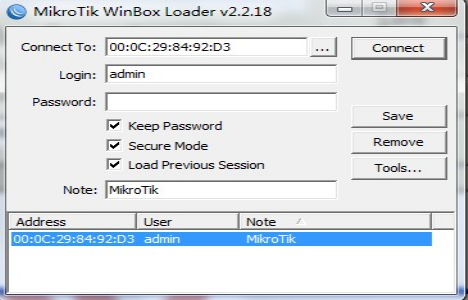
\includegraphics[width=.7\textwidth]{pic/winbox.png}
  \caption{winbox登录界面}
  \label{fig:winbox} 
\end{figure}

MAC-telnet是在路由器没有IP地址的情况下或者配置防火墙参数后无法连接,通过路由器网卡MAC地址登
陆的方式远程连接到路由器, MAC-telnet仅能使用在来自同一个广播域中(因此在网络中不能有路由的存
在),路由器的网卡应该被启用。注意,在winbox中通过MAC地址连接路由器的功能,并内置了探测工具。
这样在管理员忘记或复位了路由器后,同样可以通过 MAC 登录到 routerOS 上,进行图形界面操作

\subsection{winbox 图形操作界面}

Winbox 控制台适用于 mikrotik routerOS 的管理和配置,使用图形管理和配置,使用它型管理接
口(GUI)。通过连接到 mikrotik 路由器的 HTTP(TCP 80 端口)欢迎界面下载 Winbox.exe 可行文件,下
载并保存在你的 windows 中,之后直接在你windows 电脑上运行 Winbox.exe 文件。

\begin{itemize}
\item
\includegraphics{pic/winbox1.png}搜索和显示 MNDP (mikrotik Neighbor discovery
  protocol) 或 CDP(cisco discovery protocol)设备,可以通过该功能键搜索同一子网
  内 mikrotik 和 cisco设备,并能通过 MAC 地址登陆到 mikrotik routerOS 进行操作。
\item 
\includegraphics{pic/winbox2.png}通过指定的 IP 地址(默认端口为 80,不许特别指定,如果你
  修改了端口需要对具体访问端口做自定)或 MAC 地址(如果路由器在同一子网内)登陆路由器。
\item 
\includegraphics{pic/winbox3.png}保存当前连接列表(当需要运行它们时,只需双击)。
\item 
\includegraphics{pic/winbox4.png}删除从列表中选择的项目。
\item 
\includegraphics{pic/winbox5.png}所有列表中的项目,清除在本地的缓存,从 Winbox 文件导入
  地址或导出为 Winbox 文件。
\item 
\includegraphics{pic/winbox6.png}Secure mode (安全模式):提供保密并
  在 Winbox 和routerOS 之间使用 TLS(transport layer security)协议; Keep password(保存密码):保
  存密码到本地磁盘的文本文件中。
\end{itemize}

\subsection{MAC 层访问(telnet 与 winbox)}

通过MAC地址进行链接是用来访问没有设置IP地址的routerOS路由设备,这种连接类似于IP地址
连接,通过MAC地址仅在限于2台mikrotik routerOS路由器之间进行, 操作路径: \verb|/tool/mac-server|。

\subsection{常用命令信息}
在任何操作目录使用‘?’都可用获在当前目录中的命令信息。
\begin{multicols}{2}
  \begin{description}
  \item[log/] --- 系统日志
  \item[Quit]---退出控制台
  \item[Radius/]---客户端设置
  \item[Certificate/]---授权管理
  \item[Special-login/]---特殊登陆用户
  \item[Ping-ping] ---命令
  \item[Setup]---基本的系统设置
  \item[Interface/]---接口配置
  \item[Password]---修改密码
  \item[Undo]---撤销以前操作
  \item[Port/]---串口控制
  \item[User/]---用户管理
  \item[System/]---系统信息和应用程序
  \item[Ip/-ip] ---选项
  \item[Tools/]---工具
  \item[Routing]---各种路由协议设置
  \item[..]---回到根目录
  \item[Address/]---地址管理
  \item[Route/]---路由管理
  \item[Firewall/]---防火墙管理
  \item[DHCP-client]---DHCP 客户端设置
  \item[DHCP-serner/]---DHCP 服务设置
  \item[Hotspot/-hotspot] ---管理
  \item[Pool-ip] ---地址池
  \end{description}
\end{multicols}

一个指令或一个变量参数不需要完整的输入, 如是含糊不清的指令或变量参数需要完整的输输
入 interface 时,你只要输入 in 或 int,需要显示完整的指令可以使用[tab]键通过指令的组合,可以在
当前的目录执行在不同目录操作

\section{配置步骤}

基本配置完成以后需要配置我们需要的ROS,对于酒店的特殊需求,我自己配置了一份ROS配置文件,
这样的好处是可以批量配置路由器,不用每次手工配置,步骤如下:
\begin{enumerate}
\item 使用winbox登录ROS,输入用户名密码。
\item 鼠标点击New Terminal,出现一个终端,复制配置文件backup.rsc(见附录~\ref{sec:ros-script})。
\item 鼠标放到终端上点击粘贴。
\item 配置成功。
\item 配置文件详见附录~\ref{sec:ros-script}。
\end{enumerate}




%%% Local Variables: 
%%% mode: latex
%%% TeX-master: "../thesis"
%%% End: 
  %%配置ROS路由器(调整了一下位置,更合理)
\chapter{网络拓扑设计}
%\label{cha:topology}

\section{设计要求}
酒店的外网接ROS的eth0口内网接eth1口,对所有交换机使用hotspot认证,酒店员工办公室的电脑、前
台电脑、特殊用户电脑不需要认证,其他普通用户电脑都需要进行认证。该集成的系统放到酒店一楼的
前台处给客户刷卡取纸条,系统只需要在前台接入酒店内网即可。对酒店普通用户限速$400K$,办公室限
速$600K$,特殊帐号不限速。用户两小时内不上网自动下线。

\subsection{拓扑设备}

\begin{itemize}
\item Raspberry Pi(树莓派),刷卡器,POS打印机三者集成为一个整体,接到一楼网络的前台处。
\item 只需把树莓派接入酒店内网即可工作。
\item 总交换机即为我们的ROS路由,通过该总路由即可管理整个酒店网络
\item 比如一楼的用户要上网,通过刷卡然后取走纸条即可上网
\item 树莓派实时控制ROS路由
\end{itemize}

\subsection{拓扑结构}

这里显示了一楼前台处的树莓派+刷卡器+打印机三者为一个整体,连接外网的是ROS,ROS的eth1接入酒
店内网交换机。

其他终端用户上网都需要经过ROS的认证,通过到前台刷卡然后如果是入住酒店打印机打印出一张纸条,
客户取走纸条后接入酒店网络弹出认证界面,按照纸条上的用户名密码输入上网。

客户退房的时候在刷一次卡,这次打印机不会出纸条,听到嘀的一声后就注销了,纸条上的用户名和密
码作废。

通过在ROUTER OS中设置IP$\rightarrow$Hotspot$\rightarrow$Ip Bindings设置不需要认证的ip,但是
对于要批量设置的话可以使用其中一个不需要认证的ip接入办公室的路由器,办公室就不用经过认证了,
办公室限速$600K$只需要限制这一个ip的网速就可以了。对于普通用户的限速在Queues里面写规则限制。

在Queues里面写限速规则
\begin{enumerate}
\item ROS单IP限速
  \begin{enumerate}
  \item 首先登陆WINBOX,点击QUEUES,这个就是限速窗口,现在是空白的,再点击“红色+号”新建一个
    限速规则。
  \item 名字自己起,最好是一看就明白的,target upload:目标上传;target download:目标下载。
    这里要说明一下,在ROS里表达的流量值单位是位(bit),而我们平时说的申请了$2M$的ADSL,这
    个$2M$,单位也是位(bit),但是我们说的下载速度多少$K$,指的单位是字节,它们之间的比例
    是:8位(bit)$=$1字节,所以,上传$128k/8=15K$(请注意大小写:$k*8=K$)。下面还可以设置
    每个星期几限速,全打上就是每一天都限的意思。
  \item 当我们设置完了限制的速度后,我们还要设置要限制的电脑IP,才能实现效果哦。点
    击advanced(高级)栏,在dst. address处输入你要限制速度的IP地址,然后点OK完成。
  \item ROS限速的确很好用,限了多少就是多少,非常准确的。
  \end{enumerate}
\item ROS网段限速
  \begin{enumerate}
  \item 首先登陆WINBOX,点击:system-scripts
  \item 通过脚本来对整个网段限速,先点“红色+号”,新建一个脚本,名字你喜欢,在SOURCE处粘贴源代码   
    \begin{minted}[fontsize=\small,
      linenos=true,numbersep=2pt,
      frame=leftline,framesep=3pt,rulecolor=\color{lightgray},
      xleftmargin=10pt
      ]{bash}
      :for myip from 2 to 250
      do={
        /queue simple add name=(“限192.168.1.” . $myip . “”)
        target-address=(“192.168.1.” . $myip . “/32″)
        limit-at=0/0 max-limit=150000/1024000
      }
    \end{minted}
  \item 即可以192.168.1.2-250限速
  \item 创建了脚本,还要运行才能生效。选中要运行的脚本,再点击RUN…,这样整个网段都可以实现
    统一限速了。
  \end{enumerate}
\end{enumerate}

酒店网络拓扑如图~\ref{fig:hotel}所示。注意,这里仅说明了酒店的一楼网络,其他楼层同样需要经
过认证才可以上网,树莓派接入酒店内网任意位置都可以进行啥卡认证,客户的笔记本的电脑、PC、智
能手机都需要认证上网,办公室的位置没有标出。

\begin{figure}
  \centering
  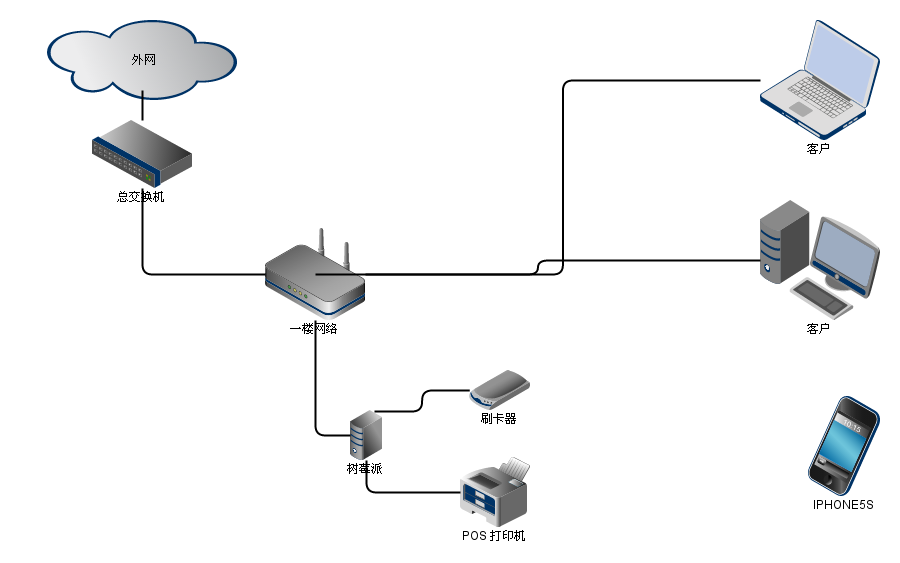
\includegraphics[width=.9\textwidth]{pic/hotel.png}
  \caption{酒店拓扑}
  \label{fig:hotel}
\end{figure}

%%% Local Variables: 
%%% mode: latex
%%% TeX-master: "../thesis"
%%% End: 
  %%网络拓扑设计
\chapter{软件方案设计}
%\label{cha:design}

\section{软件需求分析}

通过查阅资料和进行实地勘察发现,WIFI网络的管理处于一种非常不稳定的现
象,蹭网现象的频繁发生,网络资源的大量的浪费,配置的繁琐。消费客户入住酒店过程中,询问
帐号和密码的次数过多,给前台工作人员带来了工作力度,也给消费客户带来了诸多
的不便。针对这些情况,我们提出了设计一种能够达到自动化管理WIFI上网,防止蹭网和减少工作力度的软
件,该软件还可以带来广告效应和增值服务。

\section{关于Raspberry Pi}

Raspberry Pi是一个信用卡大小的电脑,可接入TV和键盘。这是一个能够在电子项目中使用的小容量PC,
同时可以做到像你的普通笔记本电脑一样的事情,诸如电子表格,文档处理和游戏。 它还能播放高清
晰度视频。我们希望看到全世界的孩子都使用它学习编程\cite{pie}。

\subsection{快速指南}
摘自《树莓派快速入门手册》(Rasperry Pi Quick Start Guide,
\url{http://www.raspberrypi.org/help/quick-start-guide/}):

\subsubsection{需要的硬件}

\begin{figure}[h]
  \centering
  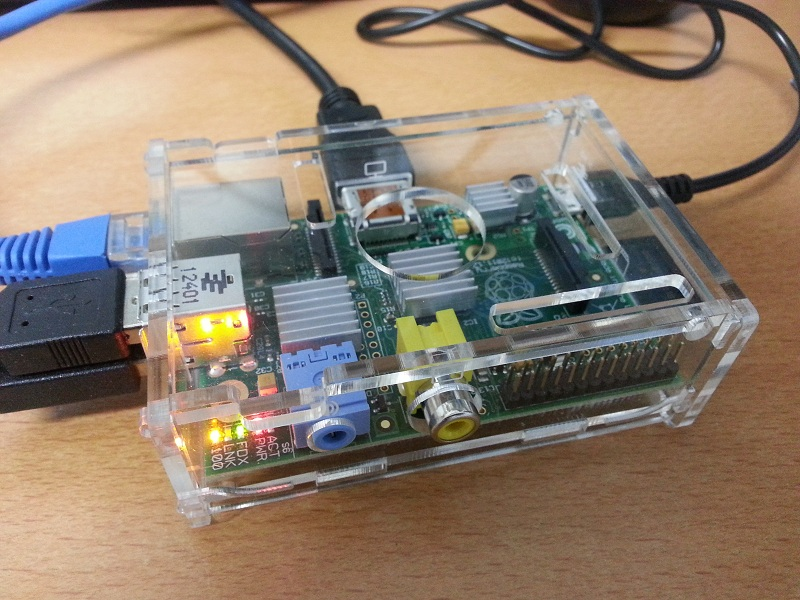
\includegraphics[width=.6\textwidth]{pic/real}
  \caption{树莓派实物图}
  \label{fig:real}
\end{figure}

图~\ref{fig:real}所示就是我们使用的树梅派。连接树梅派的还有如下一些硬件设备:
\begin{itemize}
\item SD卡一张(我们选用的是兼容树莓派的SanDisk卡 见附录~\ref{sec:sdcard})
\item HDMI高清线,VGA转接头,网线
\item 键盘鼠标
\item 电源
\end{itemize}

树莓派的物理结构如图~\ref{fig:structure}所示。

\begin{figure}
  \centering
    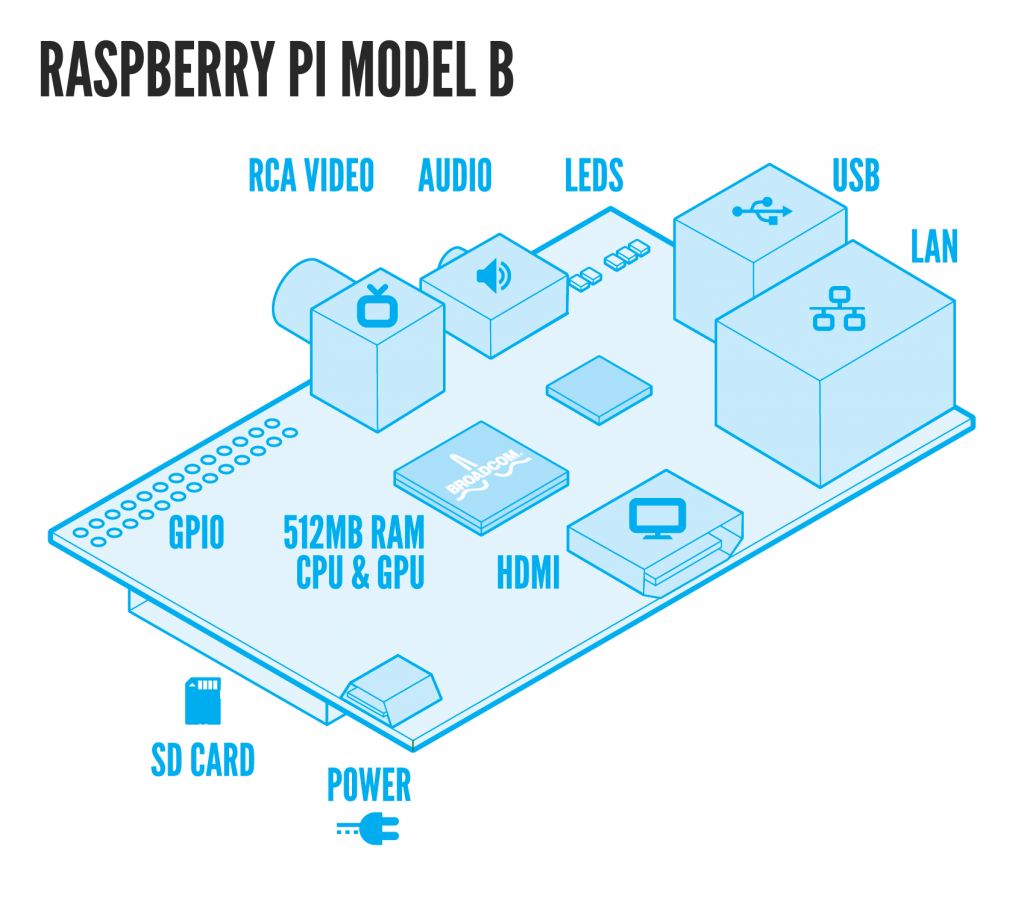
\includegraphics[width=.7\textwidth]{pic/structure}
  \caption{树莓派结构图}
  \label{fig:structure}
\end{figure}

\subsubsection{树莓派的硬件连接}

\begin{enumerate}
\item 首先将SD卡插入在树莓派上的SD卡插槽,只有一种方式插入。
\item 接下来,把usb键盘和usb鼠标插入树莓派自带的两个usb口上。
\item 确保你的显示器是开着的,接着你需要选择你的接入方式(HDMI或者DVI等等)。
\item 接着把使用树莓派的HDMI高清线接入树莓派,使用转接头接显示器的VGA插口。
\item 如果你希望你的树莓派能够联网,插入网线到网口,就在usb口旁边,如果不要联网则跳过此步。
\item 这时你应当很高兴你已经接好了所有的线以及插入了需要的SD卡,最后一部就是接入电源,树莓
  派就起来了。
\end{enumerate}

\subsubsection{登录树莓派}

\begin{enumerate}
\item 当你的树莓派已经完成启动进程后,一个登录提示符将会显示出来。默认登录树莓派的用户名
  是\verb|pi| 密码是 \verb|raspberrypi|。注意:当你输入密码的时候你看不到密码,这是linux系
  统的安全特性。
\item 在你成功登录以后,你将会看到这样的命令提示符 \verb|pi@raspberrypi~$|。
\item 要进入图形化的操作界面,输入\verb|startx|然后回车,一个漂亮的用户界面就出来了。
\end{enumerate}

\section{PYTHON模块}

\subsection{流程图}
\label{sec:desc}

\begin{figure}%[h]
  \centering
  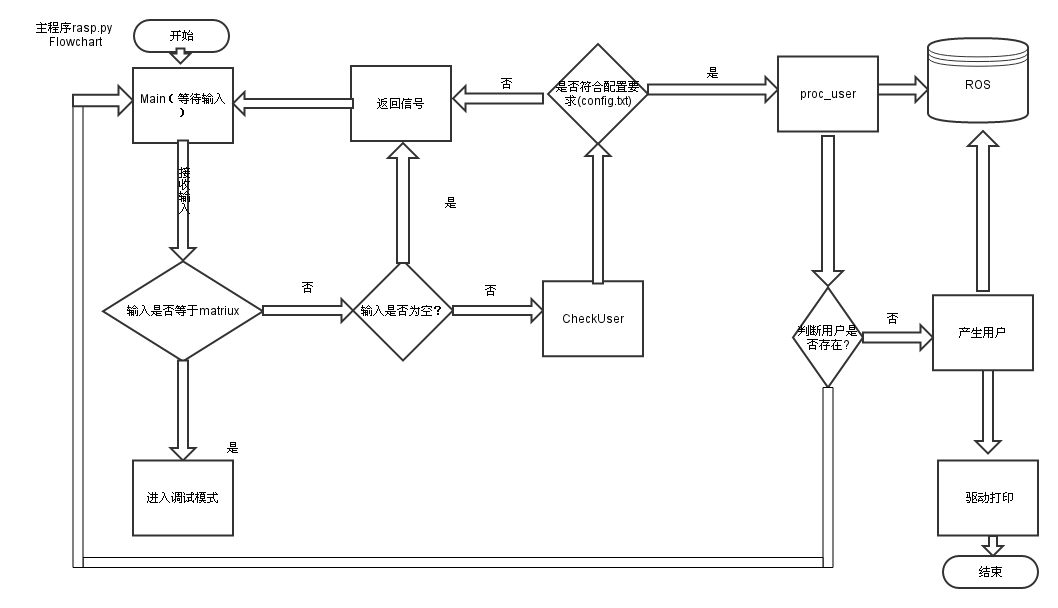
\includegraphics[width=.7\textwidth]{pic/flowchart}
  \caption{主流程图}
  \label{fig:struct}
\end{figure}

整个系统的工作流程如图\ref{fig:struct}所示。
\begin{enumerate}
\item 主程序开始$\rightarrow$进入main函数等待用户的输入(只有刷卡作为输入)。
\item 接收用户输入判断是否等于matriux(用于中断主函数等待输入的状态,便于调试)。
\item 如果输入等于预设字符串matriux,则中断监听状态,进行调试。
\item 如果输入不等于matriux,则假定输入是用户刷卡的输入。
\item 判断该输入是否为空,如果为空则返回重新等待输入。
\item 如果不为空,使用CheckUser检查用户合法性(合法性的定义在config.cfg文件中,见代码~\ref{cha:conf.cfg-1}。)
\item 经判断不符合config.cfg则返回重新等待输入,若符合要求则调用\verb|proc_user。|
\item \verb|proc_user|首先查询ROS路由器中是否已经存在该用户,若存在则踢用户下线。若不存在则
  生成新用户信息,存入ROS。
\item 存入ROS成够后调用打印机打印用户名和密码给用户上网使用。
\item 继续等待其他输入$\rightarrow$结束。
\end{enumerate}

\subsection{系统整合}
%\label{sec:integrate}

\begin{enumerate}
\item 安装PyUSB
  \begin{enumerate}
  \item 从Sourceforge\footnote{\url{http://sourceforge.net/}}上面下载最新的\verb|tarbell|
  \item \verb|unzip pyusb*.zip|
  \item \verb|cd pyusb*|
  \item \verb|python setup.py build|
  \item \verb|sudo python setup.py install|
  \end{enumerate}
\item 安装\verb|escpos|
  \begin{enumerate}
  \item \verb|wget http://python-escpos.googlecode.com/files/python-escpos-1.0.tgz|
  \item \verb|tar zxvf python-escpos-1.0.tgz|
  \item \verb|cd python-escpos-1.0|
  \item \verb|python setup.py build|
  \item \verb|sudo python setup.py install|
  \end{enumerate}
\item 安装其他软件:\verb|apt-get install python-imaging python-usb python2.7-usbtc08 python-serial|
\item PYTHON编码完成后在Raspberry Pi上测试
\item 各个程序模块已经能够在Raspberry Pi的linux系统下运行
\item 定制系统开机脚本,开机自动运行PYTHON程序
\item 测试系统稳定性
\end{enumerate}

\subsection{功能函数}

表~\ref{tab:functions}列出了程序中主要的一些函数以及函数对应的用法。

\begin{longtable}{l|l}
  \caption{函数说明}\\\hline
  函数 & 功能 \\\hline\endfirsthead
  \caption{函数说明(续)}\\\hline\endhead
  getAdminInfo & 获取admin用户的信息\\
  getNewPwd & 通过给定字符串随机构造新密码\\
  checkUser & 检查用户的合法性,通过config文件检查,返回用户名\\
  \verb|proc_user| & 写入ros数据库,产生用户名和密码\\
  getpass & termios监听程序,持续监听刷卡获得的卡号\\
  getCardNum & 刷卡后获得卡号\\
  termios.tcgetattr & 获取文件描述符\\
  termios.tcsetattr & 设置文件描述符\\
  ros.getUserlist & 获取用户列表\\
  ros.delUser & 删除用户\\
  ros.addNewUser & 添加用户\\
  rasprint.raspout & 打印输出\\
  Printer.Usb(0x04b8,0x0202) & 获取打印机标识、用于本地打印\\
  &用命令 “lsusb” 获取到当前打印机的”\\
  &Vendor ID” 和”Product ID”\\
  &假如获取到的是0x04b8:0×0202,\\
  main & 主程序\\
  \label{tab:functions}
\end{longtable}

%%% Local Variables: 
%%% mode: latex
%%% TeX-master: "../thesis"
%%% End: 
  %%软件方案设计
\chapter{芭堤酒店实施}
%\label{cha:shigongtu}

\section{机房}

机房实景如图~\ref{fig:back}所示。我们的ROS放在机架最上面,负责整个酒店的用户身份认证功能,
用下来性能还不错。eth0口连接酒店的外网,eth1连接酒店的总交换机,总交换机连接每层楼的交换机,
每层楼的终端都要经过ROS路由器的认证才能够上网。

\begin{figure}[h]
  \centering
    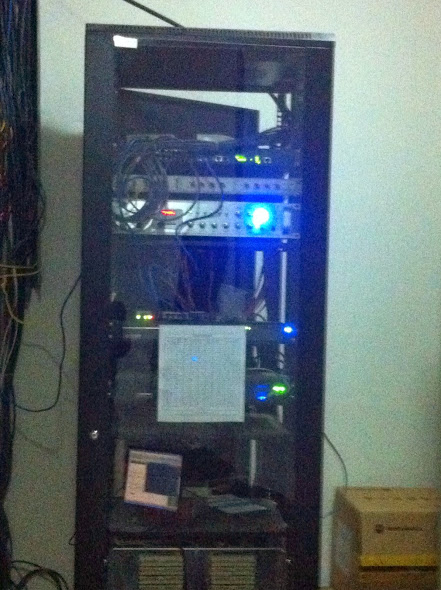
\includegraphics[width=.5\textwidth]{pic/back}
  \caption{机房}
  \label{fig:back}
\end{figure}

\section{前台}

前台实景如图~\ref{fig:front}所示。我们的树莓派+打印机+刷卡器,树莓派不需要人接触,直接放在
显示器后面。只要露出刷卡器和打印机给用户刷卡取纸就行了。刷卡器就是键盘旁边那个,打印机放在
旁边。
\begin{figure}[h]
  \centering
    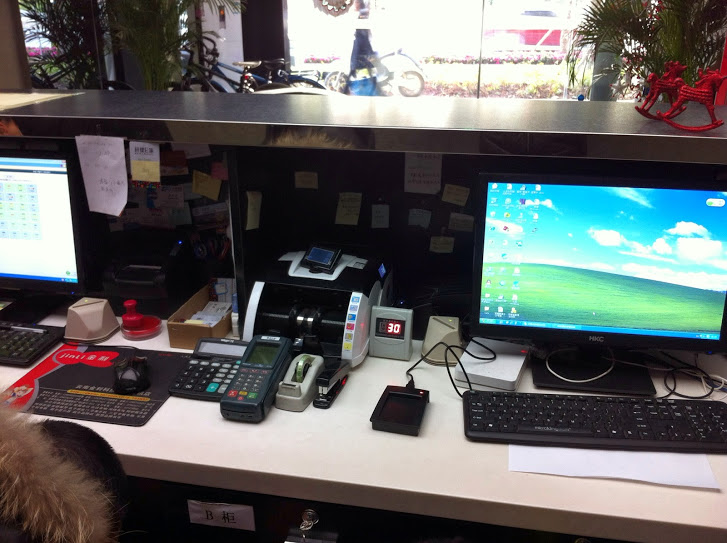
\includegraphics[width=.7\textwidth]{pic/front}
  \caption{前台}
  \label{fig:front}
\end{figure}

\section{Raspberry Pi}
%\label{sec:raspberry-pi}

图~\ref{fig:rasp}所示就是躲在角落里的树莓派,负责整个酒店的网络用户认证,总共有两个usb接口,
刷卡器接在树莓派的usb1口上,放在外面给人们刷卡,打印机接在树莓派usb2口上,放在外面打印用户
名密码,客户拿到纸条后安装纸条上的说明打开浏览器输入任意网址便会弹出带有badi酒店logo以及广
告的登录界面,然后输入用户名密码即可上网,客户离开的时候再去刷一次卡就自动下线了。另外使突
然断电也不影响酒店的网络使用,仅仅是暂时不能刷卡,只要恢复供电就又可以刷卡了。
\begin{figure}
  \centering
    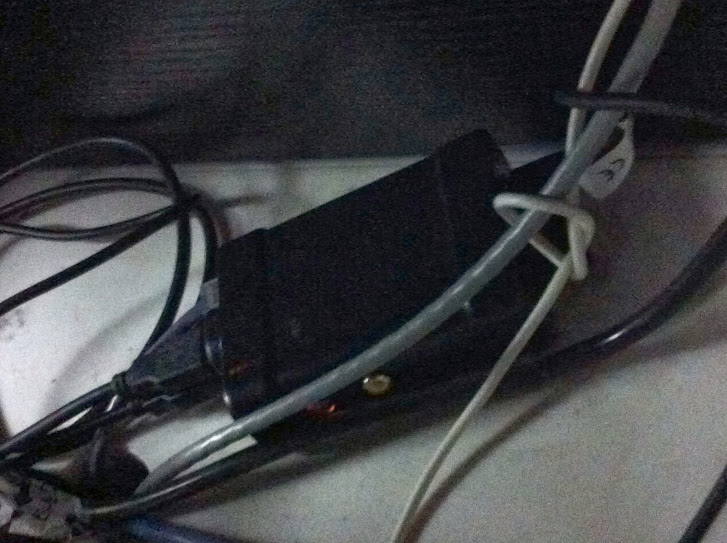
\includegraphics[width=.7\textwidth]{pic/rasp.JPG}
  \caption{树梅派}
  \label{fig:rasp}
\end{figure}

\section{实施心得}
通过在芭堤酒店的实施我得到了锻炼,我发现自己平时在学校只顾开发,从来没有和客户交流的概念,这样的话设
计出来的软件就会没有市场,我学会了要和客户交流,根据客户提出的一些建议改进
系统,比如客户提出希望操作简单方便,不要影响前台的电脑使用,我们就设想出了单独集成一套
Raspberry Pi的方案,简化了认证方式,使得工作人员不必手工去添加用户,同时不会影响前台电脑的使
用。随着使用时间的过去,根据反馈一点点改进,现在已经很稳定了,客户也很满意,产品也更成熟了。

%%% Local Variables: 
%%% mode: latex
%%% TeX-master: "../thesis"
%%% End: 
 %%施工图

%%% 正文部分到此结束。下面是『参考文献』、『指导教师简介』、『鸣谢』、『附录』
\Appendix{} % 不要动这一行!
% 下面是参考文献部分
\begin{thebibliography}{99}
\bibitem{wifi-hotspot} Geier, Eric. Wi-Fi Hotspots. Cisco Press, 2006.
\bibitem{pi-start} Richardson, Matt, and Shawn Wallace. Getting Started with Raspberry
  Pi. O'Reilly Media, Inc., 2012.
\bibitem{pi-guide} Halfacree, Gareth, and Eben Upton. Raspberry Pi User Guide. John Wiley
  \& Sons, 2012.
\bibitem{pi-python} Monk, Simon. Programming the Raspberry Pi: Getting Started with
  Python. McGraw-Hill, 2013.
\bibitem{routeros-book} 崔北亮.《Router OS 全攻略》,电子工业出版社. 2010.
\bibitem{py-ref} Beazley, David M. Python essential reference. Addison-Wesley
  Professional, 2009.
\bibitem{wxpy-act} Rappin, Noel, and Robin Dunn. wxPython in Action. Manning, 2006.
\bibitem{pie} Raspberry Pi Quick Start Guide,
  \url{http://www.raspberrypi.org/help/quick-start-guide/}
\bibitem{wikipedia-pie}Wikipedia: Raspberry Pi,
  \url{http://en.wikipedia.org/wiki/Raspberry_Pi}
\bibitem{ros} Wikipedia: MikroTik, \url{http://en.wikipedia.org/wiki/MikroTik}
\bibitem{wxpython} Wikipedia: WxPython, \url{http://en.wikipedia.org/wiki/WxPython}
\bibitem{termio} Termio Manual, \url{http://man7.org/linux/man-pages/man7/termio.7.html}
\end{thebibliography}

\advisorinfopage{} % 不要动这一行!
\acknowledgmentspage{} % 不要动这一行!

%%% 下面是附录部分。

\chapter{SD卡兼容列表}

\section{工作的SD卡}
\label{sec:sdcard}

\footnotetext{参见Working / Non-working SD cards -
  \href{http://elinux.org/RPi_SD_cards}{SD卡工作表}}
\footnotetext{本表未完全包括所有SD卡,仅列出SanDisk} 

\begin{longtable}{llllp{.1\textwidth}p{.3\textwidth}}
  \caption{SD卡工作表}\\\hline
  OK&Manufacturer&Type&Size&Class&Model\\\hline\endfirsthead
  \caption[]{SD卡工作表(续)}\\\hline\endhead
  ok&SanDisk&SD&2&?&Extreme III (BE0715105083B)\\
  % &&&&& \\
  ok&SanDisk&SD&2&2&BE0816113150D writes at 3.5 Mb/s\\
  ok&SanDisk&SD&2&4&Ultra	15 MB/s\\
  ok&SanDisk&SD&2&4&Ultra II, BE0719111366D\\
  ok&SanDisk&SD&2&6&Extreme III (BE0804212046D)	20 MB/s\\
  ok&SanDisk&SD&2&?&	SanDisk for Wii\\
  ok&SanDisk&SDHC&4&2&BH0820113475D\\
  ok&SanDisk&SDHC&4&4&SDSDB-004G-B35, BH1210821913G, SDSDB-004G-BT35\\
  ok&SanDisk&SDHC&4&4&Ultra II\\
  ok&SanDisk&SDHC&4&6&Extreme III (30 MB/s)\\
  ok&SanDisk&SDHC&4&6&Ultra SDSDH-004G-U46 - BH1136121837G,\\
  ok&SanDisk&SDHC&4&10&Extreme (BH10297143382G)\\
  ok&SanDisk&SDHC&4&10&Extreme (SDSDX-004G-X46)\\
  ok&SanDisk&SDHC&8&4&writes at ~1.5MB/s\\
  ok&SanDisk&SDHC&8&4&Ultra BI1024716014G\\
  ok&SanDisk&SDHC&8&4&SDSDB-008G-B35S / SDSDB-008G-B35\\
  ok&SanDisk&SDHC&8&4&SDSDB3-008G-A16BJ\\
  ok&SanDisk&SDHC&8&6&Ultra SDSDH-008G-U46\\
  ok&SanDisk&SDHC&8&10&Extreme\\
  ok&SanDisk&SDHC&8&10&Extreme\\
  ok&SanDisk&SDHC&8&10&Extreme Pro\\
  ok&SanDisk&SDHC&8&10&Extreme Pro\\
  ok&SanDisk&SDHC&8&10&Ultra SDSDU-008G-U46 (30 MB/s)\\
  ok&SanDisk&SDHC&8&10&Ultra SDSDU-008G-A11 (30 MB/s)\\
  ok&SanDisk&SDHC&8&10&Ultra SDSDU-008G-T11 (30 MB/s)\\
  ok&SanDisk&SDHC&8&10&Ultra SDSDU-008G-UQ46 (30 MB/s)\\
  ok&SanDisk&SDHC&16&4&SDSDB-016G-B35\\
  ok&SanDisk&SDHC&16&4&SDSDB-016G-A11\\
  ok&SanDisk&SDHC&16&6&Ultra (30MB/s) (BL1133921933G)\\
  ok&SanDisk&SDHC&16&10&Extreme\\
  ok&SanDisk&SDHC&16&10&Extreme Pro\\
  ok&SanDisk&SDHC&16&10&Ultra(30MB/s) (SDSDU-016G-U46) (SDSDU-016G-U46S)\\
  ok&SanDisk&microSDHC&16&10&Ultra microSDHC I UHS-I\\
  ok&SanDisk&SDHC&16&10&EXTREME SDHC UHS-I (SDSDX-016G-X46)\\
  ok&SanDisk&SDHC&32&4\\
  ok&SanDisk&SDHC&32&6\\
  ok&SanDisk&SDHC&32&10&Extreme (45MB/s UHS-I) (SDSDX-032G-X46)\\
  ok&SanDisk&SDHC&32&10&Ultra (30 MB/s)\\
  ok&SanDisk&SDHC&32&10&Elevate (30 MB/s) SDSDU-032G-T11\\
  ok&SanDisk&SDXC&64&10&Extreme (SDSDX-064G-X46)\\
  ok&SanDisk&SDXC&64&10&Ultra SDXC UHS-I FFP (3A114807)\\
  ok&SanDisk&microSDHC&4&2\\
  ok&SanDisk&microSDHC&4&4\\
  ok&SanDisk&microSDHC&8&2\\
  ok&SanDisk&microSDHC&8&4\\
  ok&SanDisk&microSDHC&8&4&SDSDQM-008G-B35\\
  ok&SanDisk&microSDHC&8&10&Ultra (SDSDQU-008G-U46) 30 MB/s\\
  ok&SanDisk&microSDHC&16&10&Mobile Ultra (SDSDQUA-016G-U46A)\\
  ok&SanDisk&microSDHC&32&4\\
  ok&SanDisk&microSDHC&32&10&SDSDQU-032G-U46A\\
  ok&SanDisk&microSDXC&64&6&SDSDQY-064G-A11A\\\hline{}
\end{longtable}

\chapter{配置文件}
\section{主程序配置文件(conf.cfg)}
\label{cha:conf.cfg-1}

\inputminted{python}{../src/conf.cfg}

% 见代码~\ref{cha:conf.cfg-1}。

\section{ROS配置脚本(backup.rsc)}
\label{sec:ros-script}

\inputminted{bash}{../src/backup.rsc}

\chapter{程序代码清单}

\section{pyhook函数引用}
\label{sec:pyhook}

\inputminted[fontsize=\small,
  linenos=true,numbersep=2pt,
  frame=leftline,framesep=3pt,rulecolor=\color{lightgray},
  xleftmargin=10pt
  ]{python}{../src/pyHook/Hook.py}

\section{主程序模块}
%\label{sec:main}

\inputminted[fontsize=\small,
  linenos=true,numbersep=2pt,
  frame=leftline,framesep=3pt,rulecolor=\color{lightgray},
  xleftmargin=10pt
  ]{python}{../src/rasp.py}

\section{打印模块}
%\label{sec:rasprint}

\inputminted[fontsize=\small,
  linenos=true,numbersep=2pt,
  frame=leftline,framesep=3pt,rulecolor=\color{lightgray},
  xleftmargin=10pt
  ]{python}{../src/rasprint.py}

\section{ros模块}
%\label{sec:ros}

\inputminted[fontsize=\small,
  linenos=true,numbersep=2pt,
  frame=leftline,framesep=3pt,rulecolor=\color{lightgray},
  xleftmargin=10pt
  ]{python}{../src/ros.py}

\section{readcard模块}
%\label{sec:readcard}

\inputminted[fontsize=\small,
  linenos=true,numbersep=2pt,
  frame=leftline,framesep=3pt,rulecolor=\color{lightgray},
  xleftmargin=10pt
  ]{python}{../src/readcard.py}

\section{myconf模块}
%\label{sec:myconf}

\inputminted[fontsize=\small,
  linenos=true,numbersep=2pt,
  frame=leftline,framesep=3pt,rulecolor=\color{lightgray},
  xleftmargin=10pt
  ]{python}{../src/myconf.py}


%%% Local Variables: 
%%% mode: latex
%%% TeX-master: "../thesis"
%%% End: 
   % 附录

\end{document} % 此行后面不要有任何文字。

%%% Local Variables:
%%% mode: latex
%%% TeX-master: t
%%% End:
